\section{Working hours}

\subsection{Sleep rythm}
To evaluate the significance of the punchcard in terms of sleep rhythm analysis, a small survey in a closed community has been made.
A selected group of ten people, who know each other well has been selected, for this purpose.
Furthermore a subset of four people has been chosen, which were going to be evaluated.
All ten people then needed to assign the punchcard of the chosen subset to a specific person.

To this end, three quite similar patterns, where one contributor has a very regular sleep rhythm, Graph 2 in Figure~\ref{fig:random-sleep-rhythm}, and one pattern of a practically inexistent sleep rhythm, Graph 1 in Figure~\ref{fig:random-sleep-rhythm}, have been selected.

The results of this survey where just as expected.
For the three similar graphs, no significant results could be assessed, as the assignments where more or less random.
The contributor with the irregular sleep rhythm on the other hand got correctly assigned in all in every survey.

Sadly, as such an survey needs very specific targeting and a long lead time for data collection, it could only be executed on a small set on subjects.
Anyhow the result of this survey proofs, that there exists a correlation between the structure of the punchcard and the actual commit and sleep behaviour of an contributer, even if it can only be accurately assigned in extreme cases.


\begin{figure}[H]
    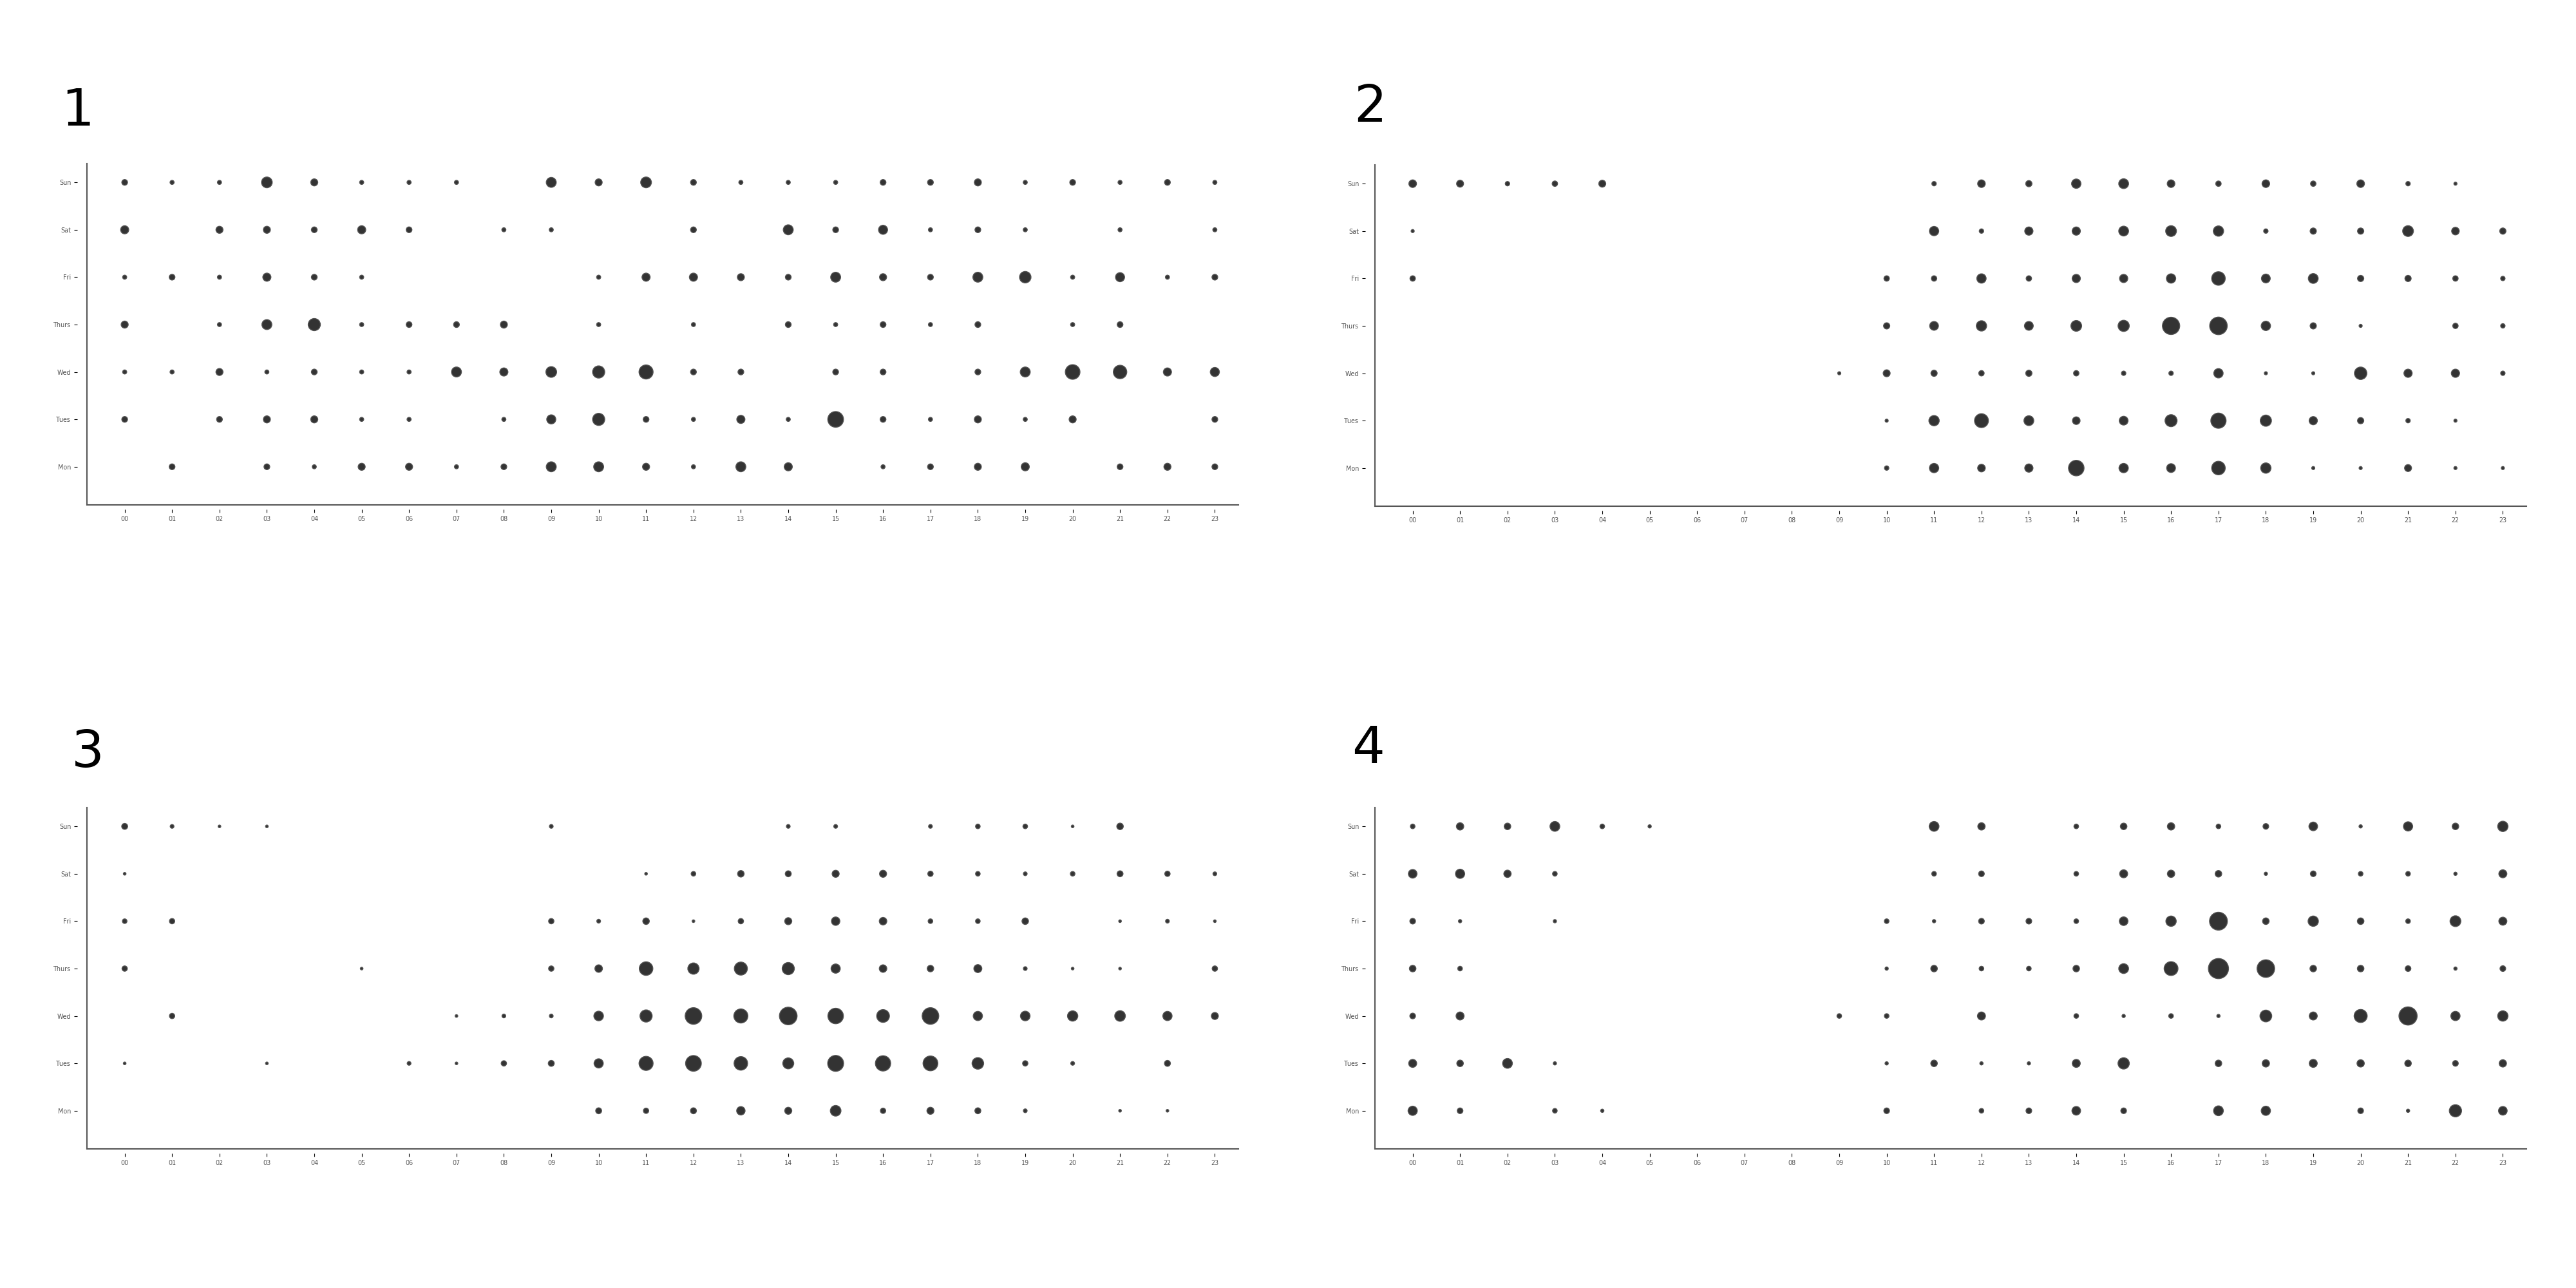
\includegraphics[scale=0.16]{./graphs/analysis/survey_combined}
    \centering
    \caption{Punchcard of an user without an irregular sleep rhythm.}\label{fig:random-sleep-rhythm}
\end{figure}

\subsection{Employee or Open-Source Contributor}
To determine whether a punchcard could be used to distinguish between an employee or an open-source contributor, the results of the clustering described in Section~\ref{punchcard-implementation} has been utilized.
For this approach two assumptions have been made.
An usual employee works between Monday and Friday during the day and only as an exception at the weekend.
An open-source developer works outside of the usual work shifts, which means early and late during weekdays and at the weekend.

For each assumption two representative clusters have been chosen and ten random persons have been selected for each cluster.
The manual verification is conducted by checking if the contributor mainly contributes to repositories which belong to the registered employee.
In case no employee exists, it is examined whether the contributor pushes to their own or open-source projects or rather to the repositories of a specific company.

\begin{figure}[H]
    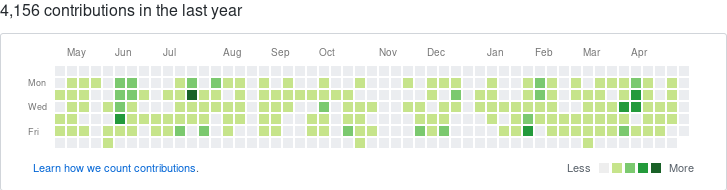
\includegraphics[scale=0.6]{./graphs/contribution-overview-alxhub}
    \centering
    \caption{Github contribution overview a Google developer with the Github nickname alxhub.}\label{fig:random-sleep-rhythm}
\end{figure}

It provides a good overview of the usual weekday work pattern over the last year and allows to quickly inspect the repositories a contributor committed to at a specific date.

\begin{figure}[H]
    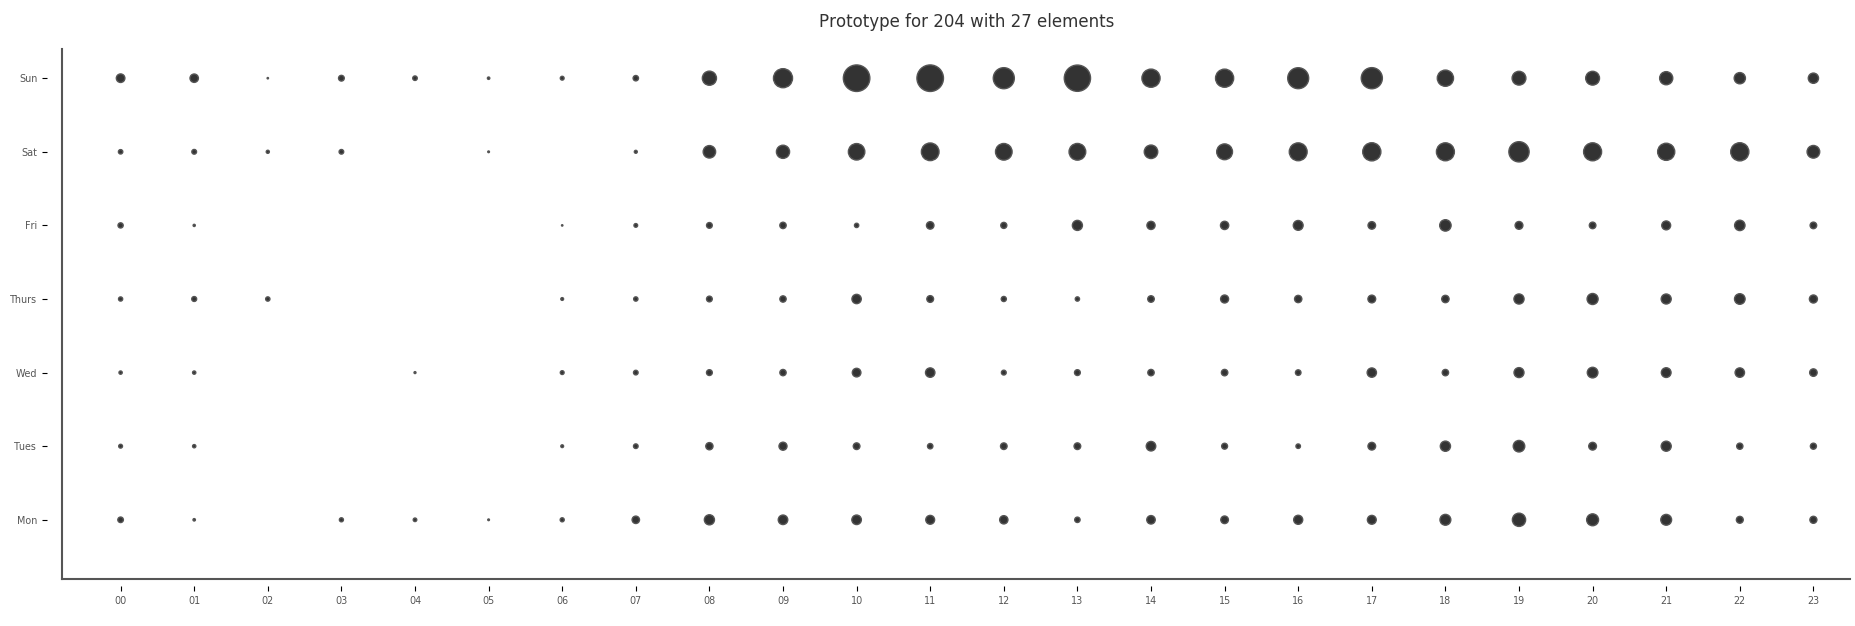
\includegraphics[scale=0.32]{./graphs/analysis-affinity/204}
    \centering
    \caption{Punchcard of an example from an affinity propagation cluster with a weekend tendency.}\label{fig:random-sleep-rhythm}
\end{figure}

The representatives for the usual five-day week commit behaviour were surprisingly accurate.
About 93\% of considered contributors were mainly working on projects of their companies, with occasional commits to their open source projects.
The remaining 7\% were either open-source developer with a very consistent commit behaviour, or it could not be determined if they work for a company.

The representatives for the leisure time commit behaviour are mostly correct as well.
About 88\% of considered contributors were irregularly contributing to either work unrelated open-source projects or their own projects.
Approximately the half of those contributors specified their employee and didn't work on their employees' projects.
The other half worked either on their own projects or on open-source projects on an irregular basis.
The remaining 12\% were either contributors working and committing to their employee's projects, but also to their own and open source projects, and employees with an untypical commit behaviour.

This analysis shows quite well, that there is a correlation between the assumed patterns and the github commit behaviour or the employment status of contributor.
Unfortunately, the evaluation process for these results is very time consuming and thereby only a relatively small sample group has been chosen.
As it is not trivial to link the employee of an contributor to all their funded projects, all verification needed to be conducted manually.

\begin{figure}[H]
    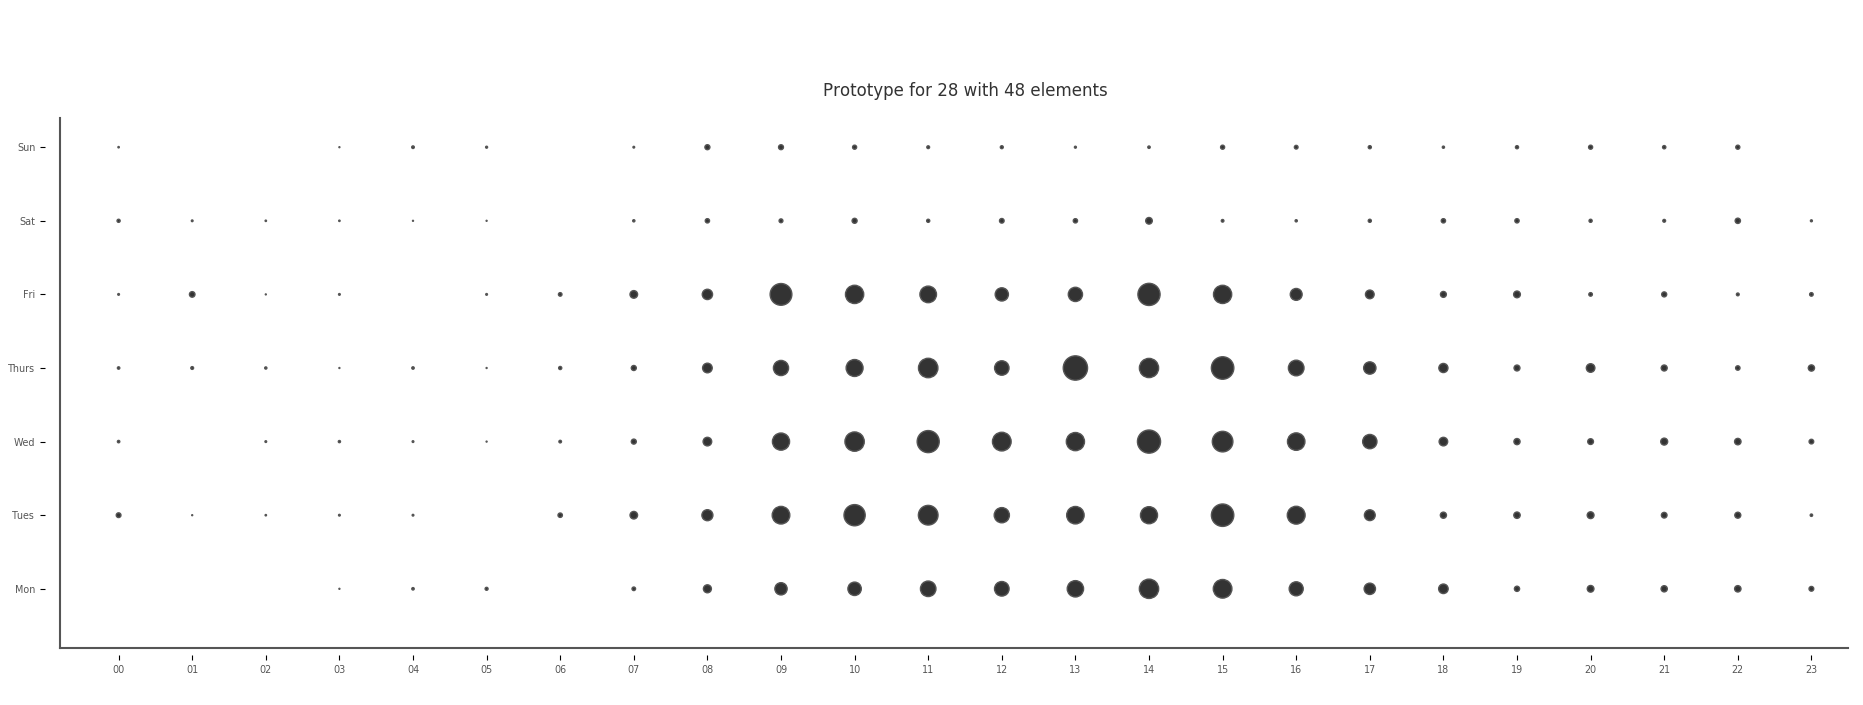
\includegraphics[scale=0.32]{./graphs/analysis-affinity/28}
    \centering
    \caption{Punchcard of an example from an affinity propagation cluster with normal work shifts.}\label{fig:random-sleep-rhythm}
\end{figure}


\subsection{Bot detection}
Another possible attack was the detection of automatically committing programs, so called \emph{bots}.
This algorithm simply detected centroids with an extremely equally distributed pattern or patterns with a spike at a specific hour.
After a manual revision of the by the algorithm detected clusters, it became apparent, that only a small subset of those clusters actually contained bots.
And even if the cluster contained bots, there were usually only one or two of them from a much larger pool of cluster members.

Detection of bots in the outliers, which were not assigned to any cluster, did not seem to be promising as well.
Manual revision of over 50 possible candidates lead to not a single bot.
After reviewing these results, I decided, that there is currently no viable approach for my data to this problem.
